\documentclass{article}
\usepackage[utf8]{inputenc}
\usepackage{tikz}
\usepackage{graphicx}
\graphicspath{ {./images/} }

\title{CS132 Quizzes - Digital Logic}
\begin{document}
\begin{center}
    \Huge\textbf{CS132 Quizzes - Digital Logic}\\
    \huge\textit{May 2021}\\
    \medskip
    \Large\textit{Josh Fitzmaurice}
\end{center}


\section{Subtract 9 from 13 in 8-bit wide two’s complement.}
13 = 00001101\\
9 = 00001001\\
flip bits\\
  = 11110110\\
add 1\\
-9 = 11110111\\
13 + (-9) = 00001101 + 11110111 = (1)00000100\\
ignore the overflow\\
13 - 9 = 00000100 = 4.

\section{Explain, with the aid of a diagram, the difference between combinatorial and sequential logic circuits.}
A combinatorial logic will give the same results given the same inputs every
time. There is no state of the circuit that can affect the output.\\
Whereas a sequential logic circuit can have a state which the circuit is in that
could mean given the same input at different times could give a different
result.\\

\begin{figure}[h]
    \centering
    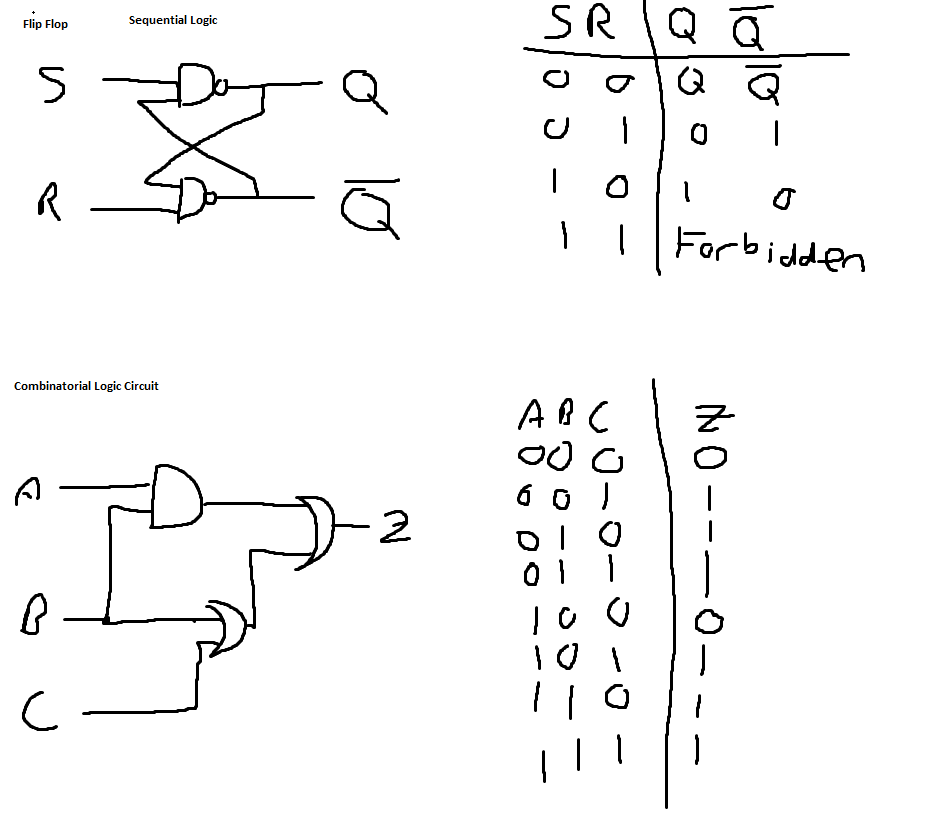
\includegraphics[width=100mm]{digitalLogic.PNG}
    \caption{examples}
    \label{fig:my_label}
\end{figure}

\section{Show the truth table for an OR gate.}
\begin{table}[h]
    \centering
    \begin{tabular}{|c|c|c|}
        A & B & Output \\
        0 & 0 & 0\\
        0 & 1 & 1\\
        1 & 0 & 1\\
        1 & 1 & 1\\
    \end{tabular}
    \caption{OR}
    \label{tab:my_label}
\end{table}

\section{Show the truth table for an XOR gate.}
\begin{table}[h]
    \centering
    \begin{tabular}{|c|c|c|}
        A & B & Output \\
        0 & 0 & 0\\
        0 & 1 & 1\\
        1 & 0 & 1\\
        1 & 1 & 0\\
    \end{tabular}
    \caption{XOR}
    \label{tab:my_label}
\end{table}

\section{Design a circuit that implements the function of an EX-OR gate using only NOT, AND and OR gates.}

\begin{figure}[h]
    \centering
    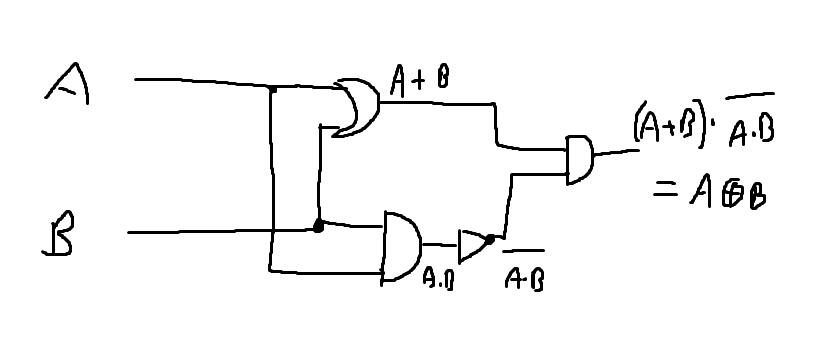
\includegraphics[width=100mm]{digitalLogic2.PNG}
    \caption{examples}
    \label{fig:my_label}
\end{figure}
\newpage
\section{Show the truth tables for a AND gate.}
\begin{table}[h]
    \centering
    \begin{tabular}{|c|c|c|}
        A & B & Output \\
        0 & 0 & 0\\
        0 & 1 & 0\\
        1 & 0 & 0\\
        1 & 1 & 1\\
    \end{tabular}
    \caption{AND}
    \label{tab:my_label}
\end{table}

\section{Design a circuit that implements the function of an OR gate using only NAND gates.}
\begin{figure}[h]
    \centering
    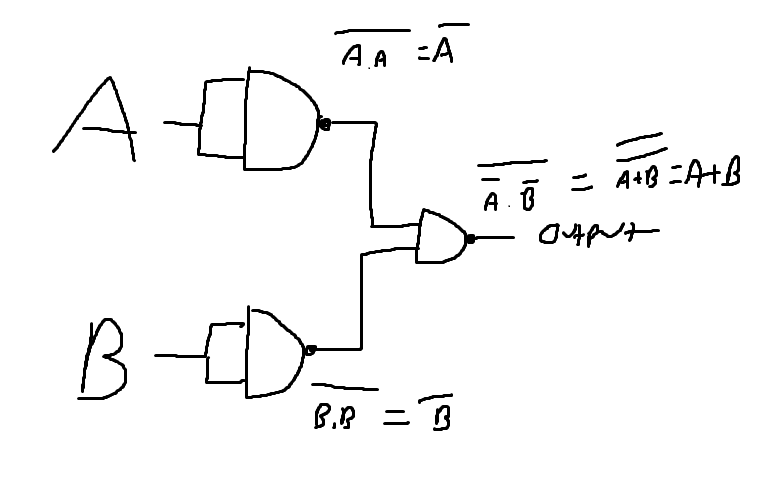
\includegraphics[width=100mm]{digitalLogic3.PNG}
    \caption{examples}
    \label{fig:my_label}
\end{figure}
\newpage
\section{Show the truth table for a 1-bit full adder.}
\begin{table}[h]
    \centering
    \begin{tabular}{|c|c|c|c|c|c|}
        A & B & Carry In & & Sum & Carry Out \\
        0 & 0 & 0 & & 0 & 0\\
        0 & 1 & 0 & & 1 & 0\\
        1 & 0 & 0 & & 1 & 0\\
        1 & 1 & 0 & & 0 & 1\\
        0 & 0 & 1 & & 1 & 0\\
        0 & 1 & 1 & & 0 & 1\\
        1 & 0 & 1 & & 0 & 1\\
        1 & 1 & 1 & & 1 & 1
    \end{tabular}
    \caption{1-bit full adder truth table}
    \label{tab:my_label}
\end{table}

\section{Design am N-bit Full Adder circuit.}
\begin{figure}[h]
    \centering
    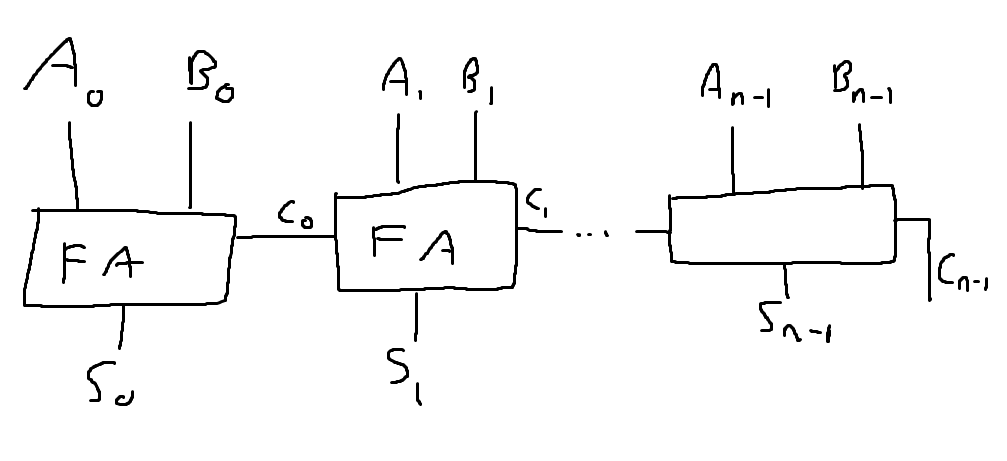
\includegraphics[width=100mm]{digitalLogic4.PNG}
    \caption{examples}
    \label{fig:my_label}
\end{figure}

\section{Explain how an N-bit Full Adder circuit can be modified to form an N-bit subtractor circuit.}
We can use the fact that a-b = a+(-b) and have a mode control line (z) that can
turn b into -b.\\\\
This can be done by flipping the bits of b and then adding 1. So we can XOR each
B in b with the control line. When z is high the bits will be flipped, otherwise
they will remain the same. Then to add the extra bit we can just use z as the
Carry In to the first 1-bit full adder.
\newpage
\section{Design an N-bit Subtractor circuit.}
\begin{figure}[h]
    \centering
    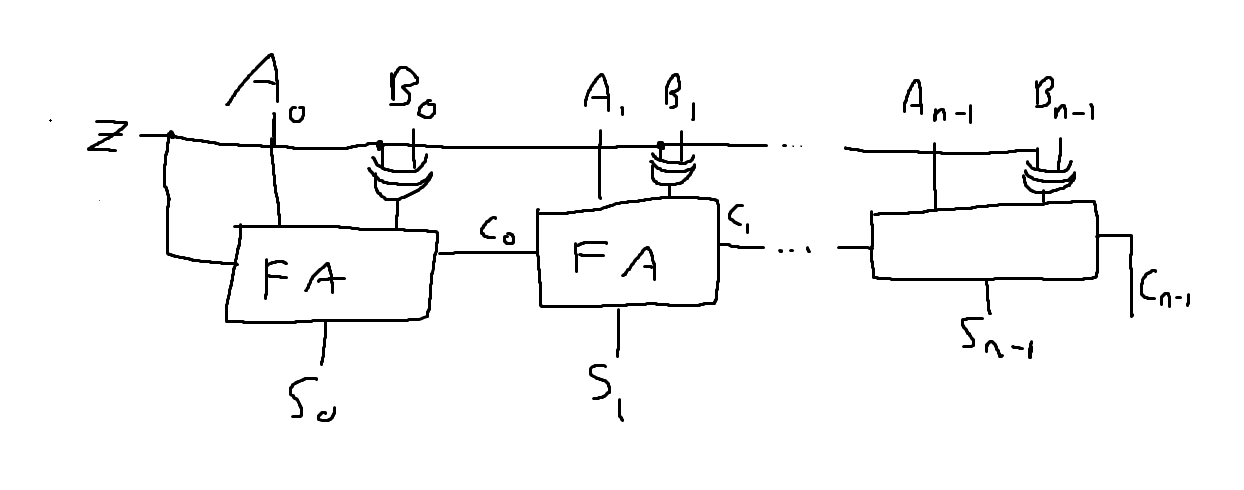
\includegraphics[width=100mm]{digitalLogic5.PNG}
    \caption{examples}
    \label{fig:my_label}
\end{figure}

\section{Explain the function of a decoder, giving an example of where a decoder might be used.}
A decoder turns n inputs into $2^n$ outputs. A decoder turns one of the outputs
on determined by the binary value of the input.\\
e.g. for an active-low decoder the truth table will be as follows:\\
\begin{table}[h]
    \centering
    \begin{tabular}{|c c|c c c c|}
        $x_0$ & $x_1$ & $y_0$ & $y_1$ & $y_2$ & $y_3$ \\
        0 & 0 & 1 & 0 & 0 & 0\\
        0 & 1 & 0 & 1 & 0 & 0\\
        1 & 0 & 0 & 0 & 1 & 0\\
        1 & 1 & 0 & 0 & 0 & 1
    \end{tabular}
    \caption{decoder}
    \label{tab:my_label}
\end{table}

Decoders are often used to address unique memory locations in a microprocessor
system
\newpage
\section{Explain the function of a multiplexer, giving an example of where a multiplexer might be used.}
A multiplexer turns n inputs into 1 output, determined by some control modes. A
multiplexer turns the output into one of the inputs determined by the control
modes.\\
multiplexer truth table for a 4-1 multiplexor (inputs are $x_0, x_1, x_2, x_3$
and control signals are $S_0, S_1$):\\
\begin{table}[h]
    \centering
    \begin{tabular}{|c c|c|}
        $S_0$ & $S_1$ & output\\
        0 & 0 & $x_0$\\
        0 & 1 & $x_1$\\
        1 & 0 & $x_2$\\
        1 & 1 & $x_3$
    \end{tabular}
    \caption{multiplexer}
    \label{tab:my_label}
\end{table}

multiplexers are used for source selection control e.g. home stereo control.

\section{Explain, using an appropriate truth table or circuit diagram, the operation of a D-Type latch.}
A D-Type latch is essentially 1 bit of memory. Depending on the current state of
the D-Type latch the input to the d-type latch will alter the output.\\
Below is the circuit diagram of a D-Type Latch
\begin{figure}[h]
    \centering
    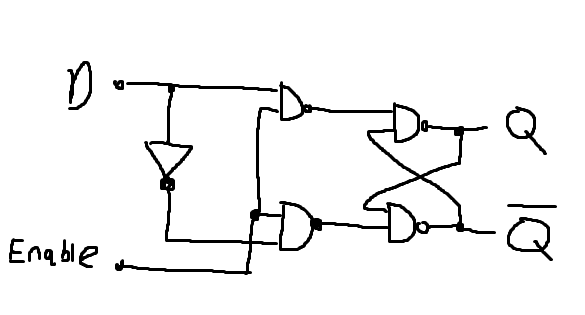
\includegraphics[width=100mm]{digitalLogic6.PNG}
    \caption{d-type latch}
    \label{fig:my_label}
\end{figure}

Below is the truth table for the d-type latch:\newpage
\begin{table}[h]
    \centering
    \begin{tabular}{|c c|c c|}
        Enable & D & Q & $\overline{Q}$\\
        \hline
        0 & 0 & Q & $\overline{Q}$\\
        0 & 1 & Q & $\overline{Q}$\\
        1 & 0 & 0 & 1\\
        1 & 1 & 1 & 0
    \end{tabular}
    \caption{D-Type latch}
    \label{tab:my_label}
\end{table}

\section{Show how D-type latches can be arranged to form an N-bit register, explaining the function of your circuit.}
\begin{figure}[h]
    \centering
    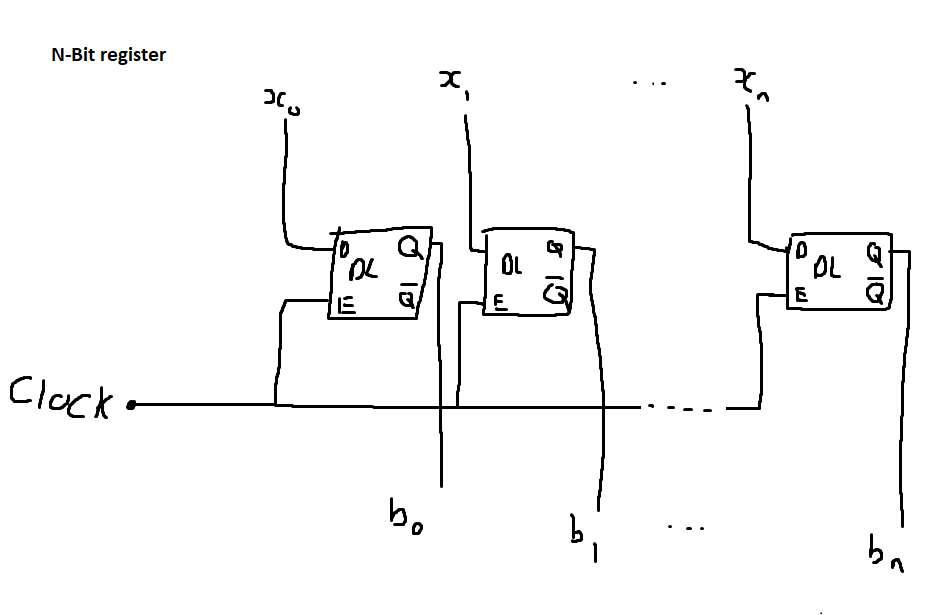
\includegraphics[width=100mm]{digitalLogic7.PNG}
    \caption{d-type latch}
    \label{fig:my_label}
\end{figure}

make note this diagram assumes the D-type latches are rising edge triggered.


\end{document}
